\documentclass[1p]{elsarticle_modified}
%\bibliographystyle{elsarticle-num}

%\usepackage[colorlinks]{hyperref}
%\usepackage{abbrmath_seonhwa} %\Abb, \Ascr, \Acal ,\Abf, \Afrak
\usepackage{amsfonts}
\usepackage{amssymb}
\usepackage{amsmath}
\usepackage{amsthm}
\usepackage{scalefnt}
\usepackage{amsbsy}
\usepackage{kotex}
\usepackage{caption}
\usepackage{subfig}
\usepackage{color}
\usepackage{graphicx}
\usepackage{xcolor} %% white, black, red, green, blue, cyan, magenta, yellow
\usepackage{float}
\usepackage{setspace}
\usepackage{hyperref}

\usepackage{tikz}
\usetikzlibrary{arrows}

\usepackage{multirow}
\usepackage{array} % fixed length table
\usepackage{hhline}

%%%%%%%%%%%%%%%%%%%%%
\makeatletter
\renewcommand*\env@matrix[1][\arraystretch]{%
	\edef\arraystretch{#1}%
	\hskip -\arraycolsep
	\let\@ifnextchar\new@ifnextchar
	\array{*\c@MaxMatrixCols c}}
\makeatother %https://tex.stackexchange.com/questions/14071/how-can-i-increase-the-line-spacing-in-a-matrix
%%%%%%%%%%%%%%%

\usepackage[normalem]{ulem}

\newcommand{\msout}[1]{\ifmmode\text{\sout{\ensuremath{#1}}}\else\sout{#1}\fi}
%SOURCE: \msout is \stkout macro in https://tex.stackexchange.com/questions/20609/strikeout-in-math-mode

\newcommand{\cancel}[1]{
	\ifmmode
	{\color{red}\msout{#1}}
	\else
	{\color{red}\sout{#1}}
	\fi
}

\newcommand{\add}[1]{
	{\color{blue}\uwave{#1}}
}

\newcommand{\replace}[2]{
	\ifmmode
	{\color{red}\msout{#1}}{\color{blue}\uwave{#2}}
	\else
	{\color{red}\sout{#1}}{\color{blue}\uwave{#2}}
	\fi
}

\newcommand{\Sol}{\mathcal{S}} %segment
\newcommand{\D}{D} %diagram
\newcommand{\A}{\mathcal{A}} %arc


%%%%%%%%%%%%%%%%%%%%%%%%%%%%%5 test

\def\sl{\operatorname{\textup{SL}}(2,\Cbb)}
\def\psl{\operatorname{\textup{PSL}}(2,\Cbb)}
\def\quan{\mkern 1mu \triangleright \mkern 1mu}

\theoremstyle{definition}
\newtheorem{thm}{Theorem}[section]
\newtheorem{prop}[thm]{Proposition}
\newtheorem{lem}[thm]{Lemma}
\newtheorem{ques}[thm]{Question}
\newtheorem{cor}[thm]{Corollary}
\newtheorem{defn}[thm]{Definition}
\newtheorem{exam}[thm]{Example}
\newtheorem{rmk}[thm]{Remark}
\newtheorem{alg}[thm]{Algorithm}

\newcommand{\I}{\sqrt{-1}}
\begin{document}

%\begin{frontmatter}
%
%\title{Boundary parabolic representations of knots up to 8 crossings}
%
%%% Group authors per affiliation:
%\author{Yunhi Cho} 
%\address{Department of Mathematics, University of Seoul, Seoul, Korea}
%\ead{yhcho@uos.ac.kr}
%
%
%\author{Seonhwa Kim} %\fnref{s_kim}}
%\address{Center for Geometry and Physics, Institute for Basic Science, Pohang, 37673, Korea}
%\ead{ryeona17@ibs.re.kr}
%
%\author{Hyuk Kim}
%\address{Department of Mathematical Sciences, Seoul National University, Seoul 08826, Korea}
%\ead{hyukkim@snu.ac.kr}
%
%\author{Seokbeom Yoon}
%\address{Department of Mathematical Sciences, Seoul National University, Seoul, 08826,  Korea}
%\ead{sbyoon15@snu.ac.kr}
%
%\begin{abstract}
%We find all boundary parabolic representation of knots up to 8 crossings.
%
%\end{abstract}
%\begin{keyword}
%    \MSC[2010] 57M25 
%\end{keyword}
%
%\end{frontmatter}

%\linenumbers
%\tableofcontents
%
\newcommand\colored[1]{\textcolor{white}{\rule[-0.35ex]{0.8em}{1.4ex}}\kern-0.8em\color{red} #1}%
%\newcommand\colored[1]{\textcolor{white}{ #1}\kern-2.17ex	\textcolor{white}{ #1}\kern-1.81ex	\textcolor{white}{ #1}\kern-2.15ex\color{red}#1	}

{\Large $\underline{12a_{0841}~(K12a_{0841})}$}

\setlength{\tabcolsep}{10pt}
\renewcommand{\arraystretch}{1.6}
\vspace{1cm}\begin{tabular}{m{100pt}>{\centering\arraybackslash}m{274pt}}
\multirow{5}{120pt}{
	\centering
	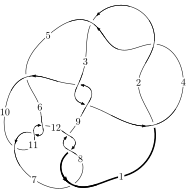
\includegraphics[width=112pt]{../../../GIT/diagram.site/Diagrams/png/1642_12a_0841.png}\\
\ \ \ A knot diagram\footnotemark}&
\allowdisplaybreaks
\textbf{Linearized knot diagam} \\
\cline{2-2}
 &
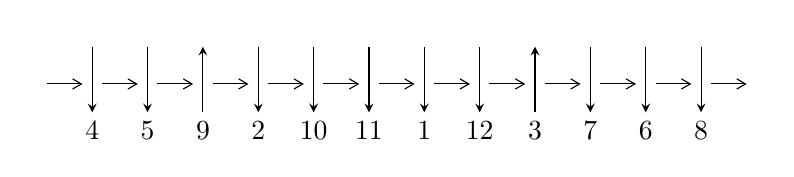
\begin{tikzpicture}[x=20pt, y=17pt]
	% nodes
	\node (C0) at (0, 0) {};
	\node (C1) at (1, 0) {};
	\node (C1U) at (1, +1) {};
	\node (C1D) at (1, -1) {4};

	\node (C2) at (2, 0) {};
	\node (C2U) at (2, +1) {};
	\node (C2D) at (2, -1) {5};

	\node (C3) at (3, 0) {};
	\node (C3U) at (3, +1) {};
	\node (C3D) at (3, -1) {9};

	\node (C4) at (4, 0) {};
	\node (C4U) at (4, +1) {};
	\node (C4D) at (4, -1) {2};

	\node (C5) at (5, 0) {};
	\node (C5U) at (5, +1) {};
	\node (C5D) at (5, -1) {10};

	\node (C6) at (6, 0) {};
	\node (C6U) at (6, +1) {};
	\node (C6D) at (6, -1) {11};

	\node (C7) at (7, 0) {};
	\node (C7U) at (7, +1) {};
	\node (C7D) at (7, -1) {1};

	\node (C8) at (8, 0) {};
	\node (C8U) at (8, +1) {};
	\node (C8D) at (8, -1) {12};

	\node (C9) at (9, 0) {};
	\node (C9U) at (9, +1) {};
	\node (C9D) at (9, -1) {3};

	\node (C10) at (10, 0) {};
	\node (C10U) at (10, +1) {};
	\node (C10D) at (10, -1) {7};

	\node (C11) at (11, 0) {};
	\node (C11U) at (11, +1) {};
	\node (C11D) at (11, -1) {6};

	\node (C12) at (12, 0) {};
	\node (C12U) at (12, +1) {};
	\node (C12D) at (12, -1) {8};
	\node (C13) at (13, 0) {};

	% arrows
	\draw[->,>={angle 60}]
	(C0) edge (C1) (C1) edge (C2) (C2) edge (C3) (C3) edge (C4) (C4) edge (C5) (C5) edge (C6) (C6) edge (C7) (C7) edge (C8) (C8) edge (C9) (C9) edge (C10) (C10) edge (C11) (C11) edge (C12) (C12) edge (C13) ;	\draw[->,>=stealth]
	(C1U) edge (C1D) (C2U) edge (C2D) (C3D) edge (C3U) (C4U) edge (C4D) (C5U) edge (C5D) (C6U) edge (C6D) (C7U) edge (C7D) (C8U) edge (C8D) (C9D) edge (C9U) (C10U) edge (C10D) (C11U) edge (C11D) (C12U) edge (C12D) ;
	\end{tikzpicture} \\
\hhline{~~} \\& 
\textbf{Solving Sequence} \\ \cline{2-2} 
 &
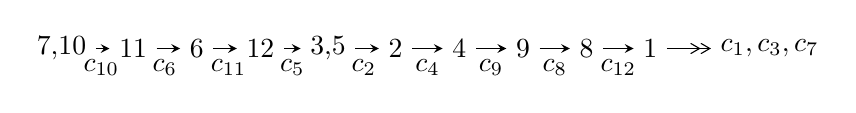
\begin{tikzpicture}[x=23pt, y=7pt]
	% node
	\node (A0) at (-1/8, 0) {7,10};
	\node (A1) at (1, 0) {11};
	\node (A2) at (2, 0) {6};
	\node (A3) at (3, 0) {12};
	\node (A4) at (65/16, 0) {3,5};
	\node (A5) at (41/8, 0) {2};
	\node (A6) at (49/8, 0) {4};
	\node (A7) at (57/8, 0) {9};
	\node (A8) at (65/8, 0) {8};
	\node (A9) at (73/8, 0) {1};
	\node (C1) at (1/2, -1) {$c_{10}$};
	\node (C2) at (3/2, -1) {$c_{6}$};
	\node (C3) at (5/2, -1) {$c_{11}$};
	\node (C4) at (7/2, -1) {$c_{5}$};
	\node (C5) at (37/8, -1) {$c_{2}$};
	\node (C6) at (45/8, -1) {$c_{4}$};
	\node (C7) at (53/8, -1) {$c_{9}$};
	\node (C8) at (61/8, -1) {$c_{8}$};
	\node (C9) at (69/8, -1) {$c_{12}$};
	\node (A10) at (11, 0) {$c_{1},c_{3},c_{7}$};

	% edge
	\draw[->,>=stealth]	
	(A0) edge (A1) (A1) edge (A2) (A2) edge (A3) (A3) edge (A4) (A4) edge (A5) (A5) edge (A6) (A6) edge (A7) (A7) edge (A8) (A8) edge (A9) ;
	\draw[->>,>={angle 60}]	
	(A9) edge (A10);
\end{tikzpicture} \\ 

\end{tabular} \\

\footnotetext{
The image of knot diagram is generated by the software ``\textbf{Draw programme}" developed by Andrew Bartholomew(\url{http://www.layer8.co.uk/maths/draw/index.htm\#Running-draw}), where we modified some parts for our purpose(\url{https://github.com/CATsTAILs/LinksPainter}).
}\phantom \\ \newline 
\centering \textbf{Ideals for irreducible components\footnotemark of $X_{\text{par}}$} 
 
\begin{align*}
I^u_{1}&=\langle 
-3 u^{28}-5 u^{27}+\cdots+8 b+3,\;-29 u^{28}-15 u^{27}+\cdots+32 a-23,\;u^{29}+15 u^{27}+\cdots+8 u^2-1\rangle \\
I^u_{2}&=\langle 
4.83718\times10^{20} u^{45}+8.97498\times10^{20} u^{44}+\cdots+9.64382\times10^{20} b+5.08979\times10^{21},\\
\phantom{I^u_{2}}&\phantom{= \langle  }5.98621\times10^{21} u^{45}+8.38005\times10^{21} u^{44}+\cdots+2.89315\times10^{21} a+6.78007\times10^{22},\;u^{46}+2 u^{45}+\cdots+36 u+9\rangle \\
I^u_{3}&=\langle 
b,\;u^2+2 a- u+3,\;u^3+2 u+1\rangle \\
I^u_{4}&=\langle 
b,\;u^3+a+u-1,\;u^4- u^3+2 u^2-2 u+1\rangle \\
I^u_{5}&=\langle 
a u+2 b- a+2 u,\;a^2- a u+a+2 u,\;u^2+1\rangle \\
\\
\end{align*}
\raggedright * 5 irreducible components of $\dim_{\mathbb{C}}=0$, with total 86 representations.\\
\footnotetext{All coefficients of polynomials are rational numbers. But the coefficients are sometimes approximated in decimal forms when there is not enough margin.}
\newpage
\renewcommand{\arraystretch}{1}
\centering \section*{I. $I^u_{1}= \langle -3 u^{28}-5 u^{27}+\cdots+8 b+3,\;-29 u^{28}-15 u^{27}+\cdots+32 a-23,\;u^{29}+15 u^{27}+\cdots+8 u^2-1 \rangle$}
\flushleft \textbf{(i) Arc colorings}\\
\begin{tabular}{m{7pt} m{180pt} m{7pt} m{180pt} }
\flushright $a_{7}=$&$\begin{pmatrix}0\\u\end{pmatrix}$ \\
\flushright $a_{10}=$&$\begin{pmatrix}1\\0\end{pmatrix}$ \\
\flushright $a_{11}=$&$\begin{pmatrix}1\\u^2\end{pmatrix}$ \\
\flushright $a_{6}=$&$\begin{pmatrix}u\\u^3+u\end{pmatrix}$ \\
\flushright $a_{12}=$&$\begin{pmatrix}u^2+1\\u^4+2 u^2\end{pmatrix}$ \\
\flushright $a_{3}=$&$\begin{pmatrix}0.906250 u^{28}+0.468750 u^{27}+\cdots+8.65625 u+0.718750\\\frac{3}{8} u^{28}+\frac{5}{8} u^{27}+\cdots-\frac{1}{8} u-\frac{3}{8}\end{pmatrix}$ \\
\flushright $a_{5}=$&$\begin{pmatrix}u^3+2 u\\u^3+u\end{pmatrix}$ \\
\flushright $a_{2}=$&$\begin{pmatrix}0.593750 u^{28}+0.0312500 u^{27}+\cdots+7.34375 u+0.781250\\\frac{1}{2} u^{28}+\frac{1}{2} u^{27}+\cdots- u-\frac{1}{2}\end{pmatrix}$ \\
\flushright $a_{4}=$&$\begin{pmatrix}0.0312500 u^{28}+0.343750 u^{27}+\cdots+8.78125 u+1.09375\\-\frac{3}{8} u^{28}-\frac{3}{8} u^{27}+\cdots-\frac{3}{8} u+\frac{1}{8}\end{pmatrix}$ \\
\flushright $a_{9}=$&$\begin{pmatrix}- u^3-2 u\\-\frac{1}{4} u^{28}-\frac{7}{2} u^{26}+\cdots-\frac{29}{4} u^3+\frac{5}{4} u\end{pmatrix}$ \\
\flushright $a_{8}=$&$\begin{pmatrix}- u\\-\frac{1}{4} u^{28}-\frac{7}{2} u^{26}+\cdots-\frac{21}{4} u^3+\frac{5}{4} u\end{pmatrix}$ \\
\flushright $a_{1}=$&$\begin{pmatrix}1\\\frac{1}{4} u^{27}+\frac{7}{2} u^{25}+\cdots+\frac{21}{4} u^2-\frac{1}{4}\end{pmatrix}$\\&\end{tabular}
\flushleft \textbf{(ii) Obstruction class $= -1$}\\~\\
\flushleft \textbf{(iii) Cusp Shapes $= \frac{153}{64} u^{28}-\frac{5}{64} u^{27}+\cdots+\frac{433}{64} u-\frac{445}{64}$}\\~\\
\newpage\renewcommand{\arraystretch}{1}
\flushleft \textbf{(iv) u-Polynomials at the component}\newline \\
\begin{tabular}{m{50pt}|m{274pt}}
Crossings & \hspace{64pt}u-Polynomials at each crossing \\
\hline $$\begin{aligned}c_{1},c_{2},c_{4}\end{aligned}$$&$\begin{aligned}
&u^{29}-4 u^{28}+\cdots+9 u-4
\end{aligned}$\\
\hline $$\begin{aligned}c_{3},c_{9}\end{aligned}$$&$\begin{aligned}
&u^{29}-3 u^{28}+\cdots-136 u-32
\end{aligned}$\\
\hline $$\begin{aligned}c_{5}\end{aligned}$$&$\begin{aligned}
&u^{29}-6 u^{28}+\cdots+256 u-64
\end{aligned}$\\
\hline $$\begin{aligned}c_{6},c_{7},c_{8}\\c_{10},c_{11},c_{12}\end{aligned}$$&$\begin{aligned}
&u^{29}+15 u^{27}+\cdots+8 u^2-1
\end{aligned}$\\
\hline
\end{tabular}\\~\\
\newpage\renewcommand{\arraystretch}{1}
\flushleft \textbf{(v) Riley Polynomials at the component}\newline \\
\begin{tabular}{m{50pt}|m{274pt}}
Crossings & \hspace{64pt}Riley Polynomials at each crossing \\
\hline $$\begin{aligned}c_{1},c_{2},c_{4}\end{aligned}$$&$\begin{aligned}
&y^{29}-30 y^{28}+\cdots+449 y-16
\end{aligned}$\\
\hline $$\begin{aligned}c_{3},c_{9}\end{aligned}$$&$\begin{aligned}
&y^{29}+21 y^{28}+\cdots+3392 y-1024
\end{aligned}$\\
\hline $$\begin{aligned}c_{5}\end{aligned}$$&$\begin{aligned}
&y^{29}-12 y^{28}+\cdots+45056 y-4096
\end{aligned}$\\
\hline $$\begin{aligned}c_{6},c_{7},c_{8}\\c_{10},c_{11},c_{12}\end{aligned}$$&$\begin{aligned}
&y^{29}+30 y^{28}+\cdots+16 y-1
\end{aligned}$\\
\hline
\end{tabular}\\~\\
\newpage\flushleft \textbf{(vi) Complex Volumes and Cusp Shapes}
$$\begin{array}{c|c|c}  
\text{Solutions to }I^u_{1}& \I (\text{vol} + \sqrt{-1}CS) & \text{Cusp shape}\\
 \hline 
\begin{aligned}
u &= \phantom{-}0.850727 + 0.156624 I \\
a &= -0.33070 - 2.13581 I \\
b &= \phantom{-}0.52738 - 1.44214 I\end{aligned}
 & -11.18250 - 6.23241 I & -15.4958 + 4.4354 I \\ \hline\begin{aligned}
u &= \phantom{-}0.850727 - 0.156624 I \\
a &= -0.33070 + 2.13581 I \\
b &= \phantom{-}0.52738 + 1.44214 I\end{aligned}
 & -11.18250 + 6.23241 I & -15.4958 - 4.4354 I \\ \hline\begin{aligned}
u &= -0.220678 + 1.200740 I \\
a &= \phantom{-}0.348620 - 0.909991 I \\
b &= \phantom{-}0.25885 - 1.75018 I\end{aligned}
 & -5.29574 + 1.64756 I & -6.64036 - 4.87433 I \\ \hline\begin{aligned}
u &= -0.220678 - 1.200740 I \\
a &= \phantom{-}0.348620 + 0.909991 I \\
b &= \phantom{-}0.25885 + 1.75018 I\end{aligned}
 & -5.29574 - 1.64756 I & -6.64036 + 4.87433 I \\ \hline\begin{aligned}
u &= -0.776315\phantom{ +0.000000I} \\
a &= \phantom{-}0.835156\phantom{ +0.000000I} \\
b &= \phantom{-}1.22191\phantom{ +0.000000I}\end{aligned}
 & -6.47257\phantom{ +0.000000I} & -15.0600\phantom{ +0.000000I} \\ \hline\begin{aligned}
u &= \phantom{-}0.762739 + 0.066975 I \\
a &= \phantom{-}0.24083 + 2.47525 I \\
b &= -0.215490 + 1.174450 I\end{aligned}
 & -4.34611 - 2.54689 I & -14.3374 + 3.8948 I \\ \hline\begin{aligned}
u &= \phantom{-}0.762739 - 0.066975 I \\
a &= \phantom{-}0.24083 - 2.47525 I \\
b &= -0.215490 - 1.174450 I\end{aligned}
 & -4.34611 + 2.54689 I & -14.3374 - 3.8948 I \\ \hline\begin{aligned}
u &= -0.389704 + 0.578994 I \\
a &= \phantom{-}0.893913 - 0.386935 I \\
b &= -0.020656 - 1.382320 I\end{aligned}
 & -6.72574 + 1.45946 I & -13.9846 - 4.7500 I \\ \hline\begin{aligned}
u &= -0.389704 - 0.578994 I \\
a &= \phantom{-}0.893913 + 0.386935 I \\
b &= -0.020656 + 1.382320 I\end{aligned}
 & -6.72574 - 1.45946 I & -13.9846 + 4.7500 I \\ \hline\begin{aligned}
u &= -0.295755 + 1.326220 I \\
a &= -0.65679 + 1.37777 I \\
b &= \phantom{-}0.152881 + 1.337510 I\end{aligned}
 & \phantom{-}3.59611 + 4.94229 I & -5.90176 - 3.25931 I\\
 \hline 
 \end{array}$$\newpage$$\begin{array}{c|c|c}  
\text{Solutions to }I^u_{1}& \I (\text{vol} + \sqrt{-1}CS) & \text{Cusp shape}\\
 \hline 
\begin{aligned}
u &= -0.295755 - 1.326220 I \\
a &= -0.65679 - 1.37777 I \\
b &= \phantom{-}0.152881 - 1.337510 I\end{aligned}
 & \phantom{-}3.59611 - 4.94229 I & -5.90176 + 3.25931 I \\ \hline\begin{aligned}
u &= -0.031725 + 1.373280 I \\
a &= \phantom{-}0.498676 + 0.750755 I \\
b &= -0.833765 + 0.932700 I\end{aligned}
 & \phantom{-}6.88971 + 1.52242 I & -3.08698 - 0.91142 I \\ \hline\begin{aligned}
u &= -0.031725 - 1.373280 I \\
a &= \phantom{-}0.498676 - 0.750755 I \\
b &= -0.833765 - 0.932700 I\end{aligned}
 & \phantom{-}6.88971 - 1.52242 I & -3.08698 + 0.91142 I \\ \hline\begin{aligned}
u &= \phantom{-}0.334857 + 1.341710 I \\
a &= -0.052463 - 0.514744 I \\
b &= \phantom{-}1.363430 + 0.335492 I\end{aligned}
 & \phantom{-}2.04714 - 8.02731 I & -6.19853 + 5.31620 I \\ \hline\begin{aligned}
u &= \phantom{-}0.334857 - 1.341710 I \\
a &= -0.052463 + 0.514744 I \\
b &= \phantom{-}1.363430 - 0.335492 I\end{aligned}
 & \phantom{-}2.04714 + 8.02731 I & -6.19853 - 5.31620 I \\ \hline\begin{aligned}
u &= -0.35253 + 1.37355 I \\
a &= \phantom{-}1.02044 - 1.34914 I \\
b &= -0.486235 - 1.297300 I\end{aligned}
 & \phantom{-}4.85486 + 10.72890 I & -4.66596 - 7.57137 I \\ \hline\begin{aligned}
u &= -0.35253 - 1.37355 I \\
a &= \phantom{-}1.02044 + 1.34914 I \\
b &= -0.486235 + 1.297300 I\end{aligned}
 & \phantom{-}4.85486 - 10.72890 I & -4.66596 + 7.57137 I \\ \hline\begin{aligned}
u &= \phantom{-}0.24683 + 1.41814 I \\
a &= \phantom{-}0.066073 + 0.309790 I \\
b &= -0.764350 - 0.100103 I\end{aligned}
 & \phantom{-}8.59031 - 5.90549 I & \phantom{-}1.11192 + 5.11469 I \\ \hline\begin{aligned}
u &= \phantom{-}0.24683 - 1.41814 I \\
a &= \phantom{-}0.066073 - 0.309790 I \\
b &= -0.764350 + 0.100103 I\end{aligned}
 & \phantom{-}8.59031 + 5.90549 I & \phantom{-}1.11192 - 5.11469 I \\ \hline\begin{aligned}
u &= \phantom{-}0.07466 + 1.44080 I \\
a &= -0.513088 - 0.364599 I \\
b &= \phantom{-}0.808356 - 0.740580 I\end{aligned}
 & \phantom{-}10.76360 - 2.89956 I & \phantom{-}0.60665 + 2.87370 I\\
 \hline 
 \end{array}$$\newpage$$\begin{array}{c|c|c}  
\text{Solutions to }I^u_{1}& \I (\text{vol} + \sqrt{-1}CS) & \text{Cusp shape}\\
 \hline 
\begin{aligned}
u &= \phantom{-}0.07466 - 1.44080 I \\
a &= -0.513088 + 0.364599 I \\
b &= \phantom{-}0.808356 + 0.740580 I\end{aligned}
 & \phantom{-}10.76360 + 2.89956 I & \phantom{-}0.60665 - 2.87370 I \\ \hline\begin{aligned}
u &= -0.40528 + 1.39829 I \\
a &= -1.16438 + 1.17876 I \\
b &= \phantom{-}0.73766 + 1.39230 I\end{aligned}
 & -1.3772 + 15.4179 I & -7.45070 - 8.08574 I \\ \hline\begin{aligned}
u &= -0.40528 - 1.39829 I \\
a &= -1.16438 - 1.17876 I \\
b &= \phantom{-}0.73766 - 1.39230 I\end{aligned}
 & -1.3772 - 15.4179 I & -7.45070 + 8.08574 I \\ \hline\begin{aligned}
u &= -0.536309\phantom{ +0.000000I} \\
a &= -0.494577\phantom{ +0.000000I} \\
b &= -0.458728\phantom{ +0.000000I}\end{aligned}
 & -1.04228\phantom{ +0.000000I} & -9.21320\phantom{ +0.000000I} \\ \hline\begin{aligned}
u &= \phantom{-}0.17794 + 1.53799 I \\
a &= \phantom{-}0.448537 - 0.057808 I \\
b &= -0.334229 + 0.884134 I\end{aligned}
 & \phantom{-}7.23806 - 6.07610 I & -7.24625 + 5.96720 I \\ \hline\begin{aligned}
u &= \phantom{-}0.17794 - 1.53799 I \\
a &= \phantom{-}0.448537 + 0.057808 I \\
b &= -0.334229 - 0.884134 I\end{aligned}
 & \phantom{-}7.23806 + 6.07610 I & -7.24625 - 5.96720 I \\ \hline\begin{aligned}
u &= -0.212154 + 0.255646 I \\
a &= -1.010790 + 0.763833 I \\
b &= \phantom{-}0.130923 + 0.622392 I\end{aligned}
 & -0.423563 + 0.810930 I & -9.27103 - 8.41081 I \\ \hline\begin{aligned}
u &= -0.212154 - 0.255646 I \\
a &= -1.010790 - 0.763833 I \\
b &= \phantom{-}0.130923 - 0.622392 I\end{aligned}
 & -0.423563 - 0.810930 I & -9.27103 + 8.41081 I \\ \hline\begin{aligned}
u &= \phantom{-}0.232774\phantom{ +0.000000I} \\
a &= \phantom{-}3.58165\phantom{ +0.000000I} \\
b &= -0.412704\phantom{ +0.000000I}\end{aligned}
 & -2.00372\phantom{ +0.000000I} & -0.355130\phantom{ +0.000000I}\\
 \hline 
 \end{array}$$\newpage\newpage\renewcommand{\arraystretch}{1}
\centering \section*{II. $I^u_{2}= \langle 4.84\times10^{20} u^{45}+8.97\times10^{20} u^{44}+\cdots+9.64\times10^{20} b+5.09\times10^{21},\;5.99\times10^{21} u^{45}+8.38\times10^{21} u^{44}+\cdots+2.89\times10^{21} a+6.78\times10^{22},\;u^{46}+2 u^{45}+\cdots+36 u+9 \rangle$}
\flushleft \textbf{(i) Arc colorings}\\
\begin{tabular}{m{7pt} m{180pt} m{7pt} m{180pt} }
\flushright $a_{7}=$&$\begin{pmatrix}0\\u\end{pmatrix}$ \\
\flushright $a_{10}=$&$\begin{pmatrix}1\\0\end{pmatrix}$ \\
\flushright $a_{11}=$&$\begin{pmatrix}1\\u^2\end{pmatrix}$ \\
\flushright $a_{6}=$&$\begin{pmatrix}u\\u^3+u\end{pmatrix}$ \\
\flushright $a_{12}=$&$\begin{pmatrix}u^2+1\\u^4+2 u^2\end{pmatrix}$ \\
\flushright $a_{3}=$&$\begin{pmatrix}-2.06910 u^{45}-2.89652 u^{44}+\cdots-63.4881 u-23.4350\\-0.501583 u^{45}-0.930646 u^{44}+\cdots-17.2611 u-5.27777\end{pmatrix}$ \\
\flushright $a_{5}=$&$\begin{pmatrix}u^3+2 u\\u^3+u\end{pmatrix}$ \\
\flushright $a_{2}=$&$\begin{pmatrix}-1.14401 u^{45}-1.45942 u^{44}+\cdots-28.8674 u-7.34206\\-0.0137503 u^{45}-0.130285 u^{44}+\cdots+2.36181 u+3.83874\end{pmatrix}$ \\
\flushright $a_{4}=$&$\begin{pmatrix}-1.43328 u^{45}-2.16999 u^{44}+\cdots-45.8330 u-15.7079\\-0.589166 u^{45}-0.982067 u^{44}+\cdots-18.1174 u-7.06307\end{pmatrix}$ \\
\flushright $a_{9}=$&$\begin{pmatrix}0.318055 u^{45}+0.101865 u^{44}+\cdots+12.9697 u+5.31725\\-0.512383 u^{45}-0.773762 u^{44}+\cdots-15.6515 u-5.26019\end{pmatrix}$ \\
\flushright $a_{8}=$&$\begin{pmatrix}-1.83572 u^{45}-2.63620 u^{44}+\cdots-63.5472 u-23.3857\\-2.15378 u^{45}-2.73806 u^{44}+\cdots-74.5169 u-28.7029\end{pmatrix}$ \\
\flushright $a_{1}=$&$\begin{pmatrix}2.15396 u^{45}+2.58331 u^{44}+\cdots+66.0693 u+22.7732\\1.03525 u^{45}+1.64133 u^{44}+\cdots+42.7004 u+14.5215\end{pmatrix}$\\&\end{tabular}
\flushleft \textbf{(ii) Obstruction class $= -1$}\\~\\
\flushleft \textbf{(iii) Cusp Shapes $= -\frac{354747019255657091139}{321460668888655555043} u^{45}-\frac{505139044943400068515}{321460668888655555043} u^{44}+\cdots-\frac{488177567341401899594}{321460668888655555043} u-\frac{3117355638652138218610}{321460668888655555043}$}\\~\\
\newpage\renewcommand{\arraystretch}{1}
\flushleft \textbf{(iv) u-Polynomials at the component}\newline \\
\begin{tabular}{m{50pt}|m{274pt}}
Crossings & \hspace{64pt}u-Polynomials at each crossing \\
\hline $$\begin{aligned}c_{1},c_{2},c_{4}\end{aligned}$$&$\begin{aligned}
&(u^{23}-3 u^{22}+\cdots- u+1)^{2}
\end{aligned}$\\
\hline $$\begin{aligned}c_{3},c_{9}\end{aligned}$$&$\begin{aligned}
&(u^{23}+u^{22}+\cdots+8 u-4)^{2}
\end{aligned}$\\
\hline $$\begin{aligned}c_{5}\end{aligned}$$&$\begin{aligned}
&(u^{23}+2 u^{22}+\cdots+18 u+9)^{2}
\end{aligned}$\\
\hline $$\begin{aligned}c_{6},c_{7},c_{8}\\c_{10},c_{11},c_{12}\end{aligned}$$&$\begin{aligned}
&u^{46}+2 u^{45}+\cdots+36 u+9
\end{aligned}$\\
\hline
\end{tabular}\\~\\
\newpage\renewcommand{\arraystretch}{1}
\flushleft \textbf{(v) Riley Polynomials at the component}\newline \\
\begin{tabular}{m{50pt}|m{274pt}}
Crossings & \hspace{64pt}Riley Polynomials at each crossing \\
\hline $$\begin{aligned}c_{1},c_{2},c_{4}\end{aligned}$$&$\begin{aligned}
&(y^{23}-23 y^{22}+\cdots-7 y-1)^{2}
\end{aligned}$\\
\hline $$\begin{aligned}c_{3},c_{9}\end{aligned}$$&$\begin{aligned}
&(y^{23}+15 y^{22}+\cdots-40 y-16)^{2}
\end{aligned}$\\
\hline $$\begin{aligned}c_{5}\end{aligned}$$&$\begin{aligned}
&(y^{23}-12 y^{22}+\cdots-450 y-81)^{2}
\end{aligned}$\\
\hline $$\begin{aligned}c_{6},c_{7},c_{8}\\c_{10},c_{11},c_{12}\end{aligned}$$&$\begin{aligned}
&y^{46}+34 y^{45}+\cdots+288 y+81
\end{aligned}$\\
\hline
\end{tabular}\\~\\
\newpage\flushleft \textbf{(vi) Complex Volumes and Cusp Shapes}
$$\begin{array}{c|c|c}  
\text{Solutions to }I^u_{2}& \I (\text{vol} + \sqrt{-1}CS) & \text{Cusp shape}\\
 \hline 
\begin{aligned}
u &= \phantom{-}0.792003 + 0.636640 I \\
a &= -0.464182 - 0.795612 I \\
b &= \phantom{-}0.107498 - 1.054050 I\end{aligned}
 & -0.12065 - 2.74438 I & -10.00137 + 3.42075 I \\ \hline\begin{aligned}
u &= \phantom{-}0.792003 - 0.636640 I \\
a &= -0.464182 + 0.795612 I \\
b &= \phantom{-}0.107498 + 1.054050 I\end{aligned}
 & -0.12065 + 2.74438 I & -10.00137 - 3.42075 I \\ \hline\begin{aligned}
u &= -0.934455 + 0.180416 I \\
a &= \phantom{-}0.01842 - 2.02427 I \\
b &= -0.63403 - 1.38420 I\end{aligned}
 & -6.36348 + 10.62070 I & -11.02627 - 6.45650 I \\ \hline\begin{aligned}
u &= -0.934455 - 0.180416 I \\
a &= \phantom{-}0.01842 + 2.02427 I \\
b &= -0.63403 + 1.38420 I\end{aligned}
 & -6.36348 - 10.62070 I & -11.02627 + 6.45650 I \\ \hline\begin{aligned}
u &= -0.415847 + 1.040410 I \\
a &= -0.783548 + 1.151140 I \\
b &= -0.308169 + 0.985429 I\end{aligned}
 & \phantom{-}2.62555 - 2.00215 I & -5.23588 + 3.62705 I \\ \hline\begin{aligned}
u &= -0.415847 - 1.040410 I \\
a &= -0.783548 - 1.151140 I \\
b &= -0.308169 - 0.985429 I\end{aligned}
 & \phantom{-}2.62555 + 2.00215 I & -5.23588 - 3.62705 I \\ \hline\begin{aligned}
u &= -0.827301 + 0.173977 I \\
a &= -0.01971 + 2.35915 I \\
b &= \phantom{-}0.383777 + 1.192290 I\end{aligned}
 & -0.03073 + 6.47771 I & -8.77780 - 6.52194 I \\ \hline\begin{aligned}
u &= -0.827301 - 0.173977 I \\
a &= -0.01971 - 2.35915 I \\
b &= \phantom{-}0.383777 - 1.192290 I\end{aligned}
 & -0.03073 - 6.47771 I & -8.77780 + 6.52194 I \\ \hline\begin{aligned}
u &= \phantom{-}0.025834 + 1.168220 I \\
a &= -1.46131 + 1.12134 I \\
b &= \phantom{-}0.441227 + 0.551458 I\end{aligned}
 & \phantom{-}1.18777 - 0.88878 I & -10.39291 - 0.92577 I \\ \hline\begin{aligned}
u &= \phantom{-}0.025834 - 1.168220 I \\
a &= -1.46131 - 1.12134 I \\
b &= \phantom{-}0.441227 - 0.551458 I\end{aligned}
 & \phantom{-}1.18777 + 0.88878 I & -10.39291 + 0.92577 I\\
 \hline 
 \end{array}$$\newpage$$\begin{array}{c|c|c}  
\text{Solutions to }I^u_{2}& \I (\text{vol} + \sqrt{-1}CS) & \text{Cusp shape}\\
 \hline 
\begin{aligned}
u &= \phantom{-}0.425501 + 1.089070 I \\
a &= -0.570025 - 0.705470 I \\
b &= -0.37388 - 1.47842 I\end{aligned}
 & -8.32991 + 1.64388 I & -13.30470 - 0.40272 I \\ \hline\begin{aligned}
u &= \phantom{-}0.425501 - 1.089070 I \\
a &= -0.570025 + 0.705470 I \\
b &= -0.37388 + 1.47842 I\end{aligned}
 & -8.32991 - 1.64388 I & -13.30470 + 0.40272 I \\ \hline\begin{aligned}
u &= \phantom{-}0.308254 + 1.133610 I \\
a &= -0.92194 - 1.29169 I \\
b &= \phantom{-}0.969482\phantom{ +0.000000I}\end{aligned}
 & \phantom{-}0.502753\phantom{ +0.000000I} & -6.32391 + 0. I\phantom{ +0.000000I} \\ \hline\begin{aligned}
u &= \phantom{-}0.308254 - 1.133610 I \\
a &= -0.92194 + 1.29169 I \\
b &= \phantom{-}0.969482\phantom{ +0.000000I}\end{aligned}
 & \phantom{-}0.502753\phantom{ +0.000000I} & -6.32391 + 0. I\phantom{ +0.000000I} \\ \hline\begin{aligned}
u &= \phantom{-}0.472378 + 0.647473 I \\
a &= -0.055315 + 1.183280 I \\
b &= -0.494865 + 0.507562 I\end{aligned}
 & \phantom{-}4.00909 - 1.37448 I & -1.29822 + 4.35124 I \\ \hline\begin{aligned}
u &= \phantom{-}0.472378 - 0.647473 I \\
a &= -0.055315 - 1.183280 I \\
b &= -0.494865 - 0.507562 I\end{aligned}
 & \phantom{-}4.00909 + 1.37448 I & -1.29822 - 4.35124 I \\ \hline\begin{aligned}
u &= \phantom{-}0.780797 + 0.120550 I \\
a &= -0.886569 - 0.462655 I \\
b &= -1.222080 - 0.199525 I\end{aligned}
 & -2.55344 - 3.99588 I & -10.60901 + 3.49800 I \\ \hline\begin{aligned}
u &= \phantom{-}0.780797 - 0.120550 I \\
a &= -0.886569 + 0.462655 I \\
b &= -1.222080 + 0.199525 I\end{aligned}
 & -2.55344 + 3.99588 I & -10.60901 - 3.49800 I \\ \hline\begin{aligned}
u &= \phantom{-}0.307733 + 1.209490 I \\
a &= \phantom{-}0.72001 + 1.31534 I \\
b &= \phantom{-}0.000983 + 1.149400 I\end{aligned}
 & -0.86138 - 1.33135 I & -11.15950 + 0. I\phantom{ +0.000000I} \\ \hline\begin{aligned}
u &= \phantom{-}0.307733 - 1.209490 I \\
a &= \phantom{-}0.72001 - 1.31534 I \\
b &= \phantom{-}0.000983 - 1.149400 I\end{aligned}
 & -0.86138 + 1.33135 I & -11.15950 + 0. I\phantom{ +0.000000I}\\
 \hline 
 \end{array}$$\newpage$$\begin{array}{c|c|c}  
\text{Solutions to }I^u_{2}& \I (\text{vol} + \sqrt{-1}CS) & \text{Cusp shape}\\
 \hline 
\begin{aligned}
u &= -0.562612 + 1.118280 I \\
a &= \phantom{-}0.694930 - 0.643080 I \\
b &= \phantom{-}0.51611 - 1.32552 I\end{aligned}
 & -3.51902 - 5.35900 I & -8.00000 + 0. I\phantom{ +0.000000I} \\ \hline\begin{aligned}
u &= -0.562612 - 1.118280 I \\
a &= \phantom{-}0.694930 + 0.643080 I \\
b &= \phantom{-}0.51611 + 1.32552 I\end{aligned}
 & -3.51902 + 5.35900 I & -8.00000 + 0. I\phantom{ +0.000000I} \\ \hline\begin{aligned}
u &= \phantom{-}0.665930 + 0.330412 I \\
a &= \phantom{-}0.671534 + 0.192645 I \\
b &= \phantom{-}0.598699 + 0.195967 I\end{aligned}
 & \phantom{-}3.01275 - 2.59653 I & -2.53697 + 3.78636 I \\ \hline\begin{aligned}
u &= \phantom{-}0.665930 - 0.330412 I \\
a &= \phantom{-}0.671534 - 0.192645 I \\
b &= \phantom{-}0.598699 - 0.195967 I\end{aligned}
 & \phantom{-}3.01275 + 2.59653 I & -2.53697 - 3.78636 I \\ \hline\begin{aligned}
u &= -0.241954 + 1.241490 I \\
a &= \phantom{-}1.62697 - 0.89642 I \\
b &= -0.308169 - 0.985429 I\end{aligned}
 & \phantom{-}2.62555 + 2.00215 I & -8.00000 + 0. I\phantom{ +0.000000I} \\ \hline\begin{aligned}
u &= -0.241954 - 1.241490 I \\
a &= \phantom{-}1.62697 + 0.89642 I \\
b &= -0.308169 + 0.985429 I\end{aligned}
 & \phantom{-}2.62555 - 2.00215 I & -8.00000 + 0. I\phantom{ +0.000000I} \\ \hline\begin{aligned}
u &= -0.708329 + 0.156769 I \\
a &= \phantom{-}0.92255 - 2.13346 I \\
b &= -0.37388 - 1.47842 I\end{aligned}
 & -8.32991 + 1.64388 I & -13.30470 - 0.40272 I \\ \hline\begin{aligned}
u &= -0.708329 - 0.156769 I \\
a &= \phantom{-}0.92255 + 2.13346 I \\
b &= -0.37388 + 1.47842 I\end{aligned}
 & -8.32991 - 1.64388 I & -13.30470 + 0.40272 I \\ \hline\begin{aligned}
u &= \phantom{-}0.004181 + 1.278050 I \\
a &= \phantom{-}0.797831 + 0.327490 I \\
b &= -0.494865 - 0.507562 I\end{aligned}
 & \phantom{-}4.00909 + 1.37448 I & \phantom{-0.000000 } 0. - 4.35124 I \\ \hline\begin{aligned}
u &= \phantom{-}0.004181 - 1.278050 I \\
a &= \phantom{-}0.797831 - 0.327490 I \\
b &= -0.494865 + 0.507562 I\end{aligned}
 & \phantom{-}4.00909 - 1.37448 I & \phantom{-0.000000 -}0. + 4.35124 I\\
 \hline 
 \end{array}$$\newpage$$\begin{array}{c|c|c}  
\text{Solutions to }I^u_{2}& \I (\text{vol} + \sqrt{-1}CS) & \text{Cusp shape}\\
 \hline 
\begin{aligned}
u &= -0.694715 + 0.088611 I \\
a &= -0.45479 - 2.70390 I \\
b &= \phantom{-}0.000983 - 1.149400 I\end{aligned}
 & -0.86138 + 1.33135 I & -11.15950 - 0.67575 I \\ \hline\begin{aligned}
u &= -0.694715 - 0.088611 I \\
a &= -0.45479 + 2.70390 I \\
b &= \phantom{-}0.000983 + 1.149400 I\end{aligned}
 & -0.86138 - 1.33135 I & -11.15950 + 0.67575 I \\ \hline\begin{aligned}
u &= -0.186653 + 1.293090 I \\
a &= -0.225783 + 0.453951 I \\
b &= \phantom{-}0.598699 - 0.195967 I\end{aligned}
 & \phantom{-}3.01275 + 2.59653 I & \phantom{-0.000000 } 0 \\ \hline\begin{aligned}
u &= -0.186653 - 1.293090 I \\
a &= -0.225783 - 0.453951 I \\
b &= \phantom{-}0.598699 + 0.195967 I\end{aligned}
 & \phantom{-}3.01275 - 2.59653 I & \phantom{-0.000000 } 0 \\ \hline\begin{aligned}
u &= -0.331769 + 1.264340 I \\
a &= \phantom{-}0.339428 - 0.762833 I \\
b &= -1.222080 + 0.199525 I\end{aligned}
 & -2.55344 + 3.99588 I & \phantom{-0.000000 } 0 \\ \hline\begin{aligned}
u &= -0.331769 - 1.264340 I \\
a &= \phantom{-}0.339428 + 0.762833 I \\
b &= -1.222080 - 0.199525 I\end{aligned}
 & -2.55344 - 3.99588 I & \phantom{-0.000000 } 0 \\ \hline\begin{aligned}
u &= \phantom{-}0.325464 + 1.311080 I \\
a &= -1.25782 - 1.25504 I \\
b &= \phantom{-}0.383777 - 1.192290 I\end{aligned}
 & -0.03073 - 6.47771 I & \phantom{-0.000000 } 0 \\ \hline\begin{aligned}
u &= \phantom{-}0.325464 - 1.311080 I \\
a &= -1.25782 + 1.25504 I \\
b &= \phantom{-}0.383777 + 1.192290 I\end{aligned}
 & -0.03073 + 6.47771 I & \phantom{-0.000000 } 0 \\ \hline\begin{aligned}
u &= -0.306328 + 1.362140 I \\
a &= -1.55159 + 0.54359 I \\
b &= \phantom{-}0.51611 + 1.32552 I\end{aligned}
 & -3.51902 + 5.35900 I & \phantom{-0.000000 } 0 \\ \hline\begin{aligned}
u &= -0.306328 - 1.362140 I \\
a &= -1.55159 - 0.54359 I \\
b &= \phantom{-}0.51611 - 1.32552 I\end{aligned}
 & -3.51902 - 5.35900 I & \phantom{-0.000000 } 0\\
 \hline 
 \end{array}$$\newpage$$\begin{array}{c|c|c}  
\text{Solutions to }I^u_{2}& \I (\text{vol} + \sqrt{-1}CS) & \text{Cusp shape}\\
 \hline 
\begin{aligned}
u &= \phantom{-}0.36850 + 1.37093 I \\
a &= \phantom{-}1.40661 + 0.98862 I \\
b &= -0.63403 + 1.38420 I\end{aligned}
 & -6.36348 - 10.62070 I & \phantom{-0.000000 } 0 \\ \hline\begin{aligned}
u &= \phantom{-}0.36850 - 1.37093 I \\
a &= \phantom{-}1.40661 - 0.98862 I \\
b &= -0.63403 - 1.38420 I\end{aligned}
 & -6.36348 + 10.62070 I & \phantom{-0.000000 } 0 \\ \hline\begin{aligned}
u &= -0.06153 + 1.44896 I \\
a &= -0.341144 - 0.682320 I \\
b &= \phantom{-}0.107498 + 1.054050 I\end{aligned}
 & -0.12065 + 2.74438 I & \phantom{-0.000000 } 0 \\ \hline\begin{aligned}
u &= -0.06153 - 1.44896 I \\
a &= -0.341144 + 0.682320 I \\
b &= \phantom{-}0.107498 - 1.054050 I\end{aligned}
 & -0.12065 - 2.74438 I & \phantom{-0.000000 } 0 \\ \hline\begin{aligned}
u &= -0.205082 + 0.466322 I \\
a &= \phantom{-}0.12875 - 3.30791 I \\
b &= \phantom{-}0.441227 - 0.551458 I\end{aligned}
 & \phantom{-}1.18777 + 0.88878 I & -10.39291 + 0.92577 I \\ \hline\begin{aligned}
u &= -0.205082 - 0.466322 I \\
a &= \phantom{-}0.12875 + 3.30791 I \\
b &= \phantom{-}0.441227 + 0.551458 I\end{aligned}
 & \phantom{-}1.18777 - 0.88878 I & -10.39291 - 0.92577 I\\
 \hline 
 \end{array}$$\newpage\newpage\renewcommand{\arraystretch}{1}
\centering \section*{III. $I^u_{3}= \langle b,\;u^2+2 a- u+3,\;u^3+2 u+1 \rangle$}
\flushleft \textbf{(i) Arc colorings}\\
\begin{tabular}{m{7pt} m{180pt} m{7pt} m{180pt} }
\flushright $a_{7}=$&$\begin{pmatrix}0\\u\end{pmatrix}$ \\
\flushright $a_{10}=$&$\begin{pmatrix}1\\0\end{pmatrix}$ \\
\flushright $a_{11}=$&$\begin{pmatrix}1\\u^2\end{pmatrix}$ \\
\flushright $a_{6}=$&$\begin{pmatrix}u\\- u-1\end{pmatrix}$ \\
\flushright $a_{12}=$&$\begin{pmatrix}u^2+1\\- u\end{pmatrix}$ \\
\flushright $a_{3}=$&$\begin{pmatrix}-\frac{1}{2} u^2+\frac{1}{2} u-\frac{3}{2}\\0\end{pmatrix}$ \\
\flushright $a_{5}=$&$\begin{pmatrix}-1\\- u-1\end{pmatrix}$ \\
\flushright $a_{2}=$&$\begin{pmatrix}-\frac{1}{2} u^2+\frac{1}{2} u-\frac{1}{2}\\u+1\end{pmatrix}$ \\
\flushright $a_{4}=$&$\begin{pmatrix}-\frac{1}{2} u^2+\frac{1}{2} u-\frac{3}{2}\\0\end{pmatrix}$ \\
\flushright $a_{9}=$&$\begin{pmatrix}1\\0\end{pmatrix}$ \\
\flushright $a_{8}=$&$\begin{pmatrix}- u\\- u^2\end{pmatrix}$ \\
\flushright $a_{1}=$&$\begin{pmatrix}1\\u+1\end{pmatrix}$\\&\end{tabular}
\flushleft \textbf{(ii) Obstruction class $= 1$}\\~\\
\flushleft \textbf{(iii) Cusp Shapes $= -\frac{25}{4} u^2+\frac{11}{4} u-\frac{71}{4}$}\\~\\
\newpage\renewcommand{\arraystretch}{1}
\flushleft \textbf{(iv) u-Polynomials at the component}\newline \\
\begin{tabular}{m{50pt}|m{274pt}}
Crossings & \hspace{64pt}u-Polynomials at each crossing \\
\hline $$\begin{aligned}c_{1},c_{2}\end{aligned}$$&$\begin{aligned}
&(u-1)^3
\end{aligned}$\\
\hline $$\begin{aligned}c_{3},c_{9}\end{aligned}$$&$\begin{aligned}
&u^3
\end{aligned}$\\
\hline $$\begin{aligned}c_{4}\end{aligned}$$&$\begin{aligned}
&(u+1)^3
\end{aligned}$\\
\hline $$\begin{aligned}c_{5}\end{aligned}$$&$\begin{aligned}
&u^3-3 u^2+5 u-2
\end{aligned}$\\
\hline $$\begin{aligned}c_{6},c_{7},c_{8}\end{aligned}$$&$\begin{aligned}
&u^3+2 u-1
\end{aligned}$\\
\hline $$\begin{aligned}c_{10},c_{11},c_{12}\end{aligned}$$&$\begin{aligned}
&u^3+2 u+1
\end{aligned}$\\
\hline
\end{tabular}\\~\\
\newpage\renewcommand{\arraystretch}{1}
\flushleft \textbf{(v) Riley Polynomials at the component}\newline \\
\begin{tabular}{m{50pt}|m{274pt}}
Crossings & \hspace{64pt}Riley Polynomials at each crossing \\
\hline $$\begin{aligned}c_{1},c_{2},c_{4}\end{aligned}$$&$\begin{aligned}
&(y-1)^3
\end{aligned}$\\
\hline $$\begin{aligned}c_{3},c_{9}\end{aligned}$$&$\begin{aligned}
&y^3
\end{aligned}$\\
\hline $$\begin{aligned}c_{5}\end{aligned}$$&$\begin{aligned}
&y^3+y^2+13 y-4
\end{aligned}$\\
\hline $$\begin{aligned}c_{6},c_{7},c_{8}\\c_{10},c_{11},c_{12}\end{aligned}$$&$\begin{aligned}
&y^3+4 y^2+4 y-1
\end{aligned}$\\
\hline
\end{tabular}\\~\\
\newpage\flushleft \textbf{(vi) Complex Volumes and Cusp Shapes}
$$\begin{array}{c|c|c}  
\text{Solutions to }I^u_{3}& \I (\text{vol} + \sqrt{-1}CS) & \text{Cusp shape}\\
 \hline 
\begin{aligned}
u &= \phantom{-}0.22670 + 1.46771 I \\
a &= -0.335258 + 0.401127 I \\
b &= \phantom{-0.000000 } 0\end{aligned}
 & \phantom{-}7.79580 - 5.13794 I & -3.98417 - 0.12290 I \\ \hline\begin{aligned}
u &= \phantom{-}0.22670 - 1.46771 I \\
a &= -0.335258 - 0.401127 I \\
b &= \phantom{-0.000000 } 0\end{aligned}
 & \phantom{-}7.79580 + 5.13794 I & -3.98417 + 0.12290 I \\ \hline\begin{aligned}
u &= -0.453398\phantom{ +0.000000I} \\
a &= -1.82948\phantom{ +0.000000I} \\
b &= \phantom{-0.000000 } 0\end{aligned}
 & -2.43213\phantom{ +0.000000I} & -20.2820\phantom{ +0.000000I}\\
 \hline 
 \end{array}$$\newpage\newpage\renewcommand{\arraystretch}{1}
\centering \section*{IV. $I^u_{4}= \langle b,\;u^3+a+u-1,\;u^4- u^3+2 u^2-2 u+1 \rangle$}
\flushleft \textbf{(i) Arc colorings}\\
\begin{tabular}{m{7pt} m{180pt} m{7pt} m{180pt} }
\flushright $a_{7}=$&$\begin{pmatrix}0\\u\end{pmatrix}$ \\
\flushright $a_{10}=$&$\begin{pmatrix}1\\0\end{pmatrix}$ \\
\flushright $a_{11}=$&$\begin{pmatrix}1\\u^2\end{pmatrix}$ \\
\flushright $a_{6}=$&$\begin{pmatrix}u\\u^3+u\end{pmatrix}$ \\
\flushright $a_{12}=$&$\begin{pmatrix}u^2+1\\u^3+2 u-1\end{pmatrix}$ \\
\flushright $a_{3}=$&$\begin{pmatrix}- u^3- u+1\\0\end{pmatrix}$ \\
\flushright $a_{5}=$&$\begin{pmatrix}u^3+2 u\\u^3+u\end{pmatrix}$ \\
\flushright $a_{2}=$&$\begin{pmatrix}-2 u^3-3 u+1\\- u^3- u\end{pmatrix}$ \\
\flushright $a_{4}=$&$\begin{pmatrix}- u^3- u+1\\0\end{pmatrix}$ \\
\flushright $a_{9}=$&$\begin{pmatrix}1\\0\end{pmatrix}$ \\
\flushright $a_{8}=$&$\begin{pmatrix}-2 u^3+u^2-3 u+3\\- u^3+u^2- u+2\end{pmatrix}$ \\
\flushright $a_{1}=$&$\begin{pmatrix}- u^3-2 u\\- u^3- u\end{pmatrix}$\\&\end{tabular}
\flushleft \textbf{(ii) Obstruction class $= 1$}\\~\\
\flushleft \textbf{(iii) Cusp Shapes $= 4 u^3+4 u-9$}\\~\\
\newpage\renewcommand{\arraystretch}{1}
\flushleft \textbf{(iv) u-Polynomials at the component}\newline \\
\begin{tabular}{m{50pt}|m{274pt}}
Crossings & \hspace{64pt}u-Polynomials at each crossing \\
\hline $$\begin{aligned}c_{1},c_{2}\end{aligned}$$&$\begin{aligned}
&(u-1)^4
\end{aligned}$\\
\hline $$\begin{aligned}c_{3},c_{9}\end{aligned}$$&$\begin{aligned}
&u^4
\end{aligned}$\\
\hline $$\begin{aligned}c_{4}\end{aligned}$$&$\begin{aligned}
&(u+1)^4
\end{aligned}$\\
\hline $$\begin{aligned}c_{5}\end{aligned}$$&$\begin{aligned}
&(u^2+u+1)^2
\end{aligned}$\\
\hline $$\begin{aligned}c_{6},c_{7},c_{8}\end{aligned}$$&$\begin{aligned}
&u^4+u^3+2 u^2+2 u+1
\end{aligned}$\\
\hline $$\begin{aligned}c_{10},c_{11},c_{12}\end{aligned}$$&$\begin{aligned}
&u^4- u^3+2 u^2-2 u+1
\end{aligned}$\\
\hline
\end{tabular}\\~\\
\newpage\renewcommand{\arraystretch}{1}
\flushleft \textbf{(v) Riley Polynomials at the component}\newline \\
\begin{tabular}{m{50pt}|m{274pt}}
Crossings & \hspace{64pt}Riley Polynomials at each crossing \\
\hline $$\begin{aligned}c_{1},c_{2},c_{4}\end{aligned}$$&$\begin{aligned}
&(y-1)^4
\end{aligned}$\\
\hline $$\begin{aligned}c_{3},c_{9}\end{aligned}$$&$\begin{aligned}
&y^4
\end{aligned}$\\
\hline $$\begin{aligned}c_{5}\end{aligned}$$&$\begin{aligned}
&(y^2+y+1)^2
\end{aligned}$\\
\hline $$\begin{aligned}c_{6},c_{7},c_{8}\\c_{10},c_{11},c_{12}\end{aligned}$$&$\begin{aligned}
&y^4+3 y^3+2 y^2+1
\end{aligned}$\\
\hline
\end{tabular}\\~\\
\newpage\flushleft \textbf{(vi) Complex Volumes and Cusp Shapes}
$$\begin{array}{c|c|c}  
\text{Solutions to }I^u_{4}& \I (\text{vol} + \sqrt{-1}CS) & \text{Cusp shape}\\
 \hline 
\begin{aligned}
u &= \phantom{-}0.621744 + 0.440597 I \\
a &= \phantom{-}0.500000 - 0.866025 I \\
b &= \phantom{-0.000000 } 0\end{aligned}
 & \phantom{-}1.64493 - 2.02988 I & -7.00000 + 3.46410 I \\ \hline\begin{aligned}
u &= \phantom{-}0.621744 - 0.440597 I \\
a &= \phantom{-}0.500000 + 0.866025 I \\
b &= \phantom{-0.000000 } 0\end{aligned}
 & \phantom{-}1.64493 + 2.02988 I & -7.00000 - 3.46410 I \\ \hline\begin{aligned}
u &= -0.121744 + 1.306620 I \\
a &= \phantom{-}0.500000 + 0.866025 I \\
b &= \phantom{-0.000000 } 0\end{aligned}
 & \phantom{-}1.64493 + 2.02988 I & -7.00000 - 3.46410 I \\ \hline\begin{aligned}
u &= -0.121744 - 1.306620 I \\
a &= \phantom{-}0.500000 - 0.866025 I \\
b &= \phantom{-0.000000 } 0\end{aligned}
 & \phantom{-}1.64493 - 2.02988 I & -7.00000 + 3.46410 I\\
 \hline 
 \end{array}$$\newpage\newpage\renewcommand{\arraystretch}{1}
\centering \section*{V. $I^u_{5}= \langle a u+2 b- a+2 u,\;a^2- a u+a+2 u,\;u^2+1 \rangle$}
\flushleft \textbf{(i) Arc colorings}\\
\begin{tabular}{m{7pt} m{180pt} m{7pt} m{180pt} }
\flushright $a_{7}=$&$\begin{pmatrix}0\\u\end{pmatrix}$ \\
\flushright $a_{10}=$&$\begin{pmatrix}1\\0\end{pmatrix}$ \\
\flushright $a_{11}=$&$\begin{pmatrix}1\\-1\end{pmatrix}$ \\
\flushright $a_{6}=$&$\begin{pmatrix}u\\0\end{pmatrix}$ \\
\flushright $a_{12}=$&$\begin{pmatrix}0\\-1\end{pmatrix}$ \\
\flushright $a_{3}=$&$\begin{pmatrix}a\\-\frac{1}{2} a u+\frac{1}{2} a- u\end{pmatrix}$ \\
\flushright $a_{5}=$&$\begin{pmatrix}u\\0\end{pmatrix}$ \\
\flushright $a_{2}=$&$\begin{pmatrix}\frac{1}{2} a u+\frac{1}{2} a+u\\-\frac{1}{2} a u+\frac{1}{2} a- u\end{pmatrix}$ \\
\flushright $a_{4}=$&$\begin{pmatrix}-\frac{1}{2} a u+\frac{1}{2} a-1\\\frac{1}{2} a u-\frac{1}{2} a+2 u\end{pmatrix}$ \\
\flushright $a_{9}=$&$\begin{pmatrix}- u\\-\frac{1}{2} a u-\frac{1}{2} a-2\end{pmatrix}$ \\
\flushright $a_{8}=$&$\begin{pmatrix}- u\\-\frac{1}{2} a u-\frac{1}{2} a+u-2\end{pmatrix}$ \\
\flushright $a_{1}=$&$\begin{pmatrix}-1\\\frac{1}{2} a u-\frac{1}{2} a+2 u\end{pmatrix}$\\&\end{tabular}
\flushleft \textbf{(ii) Obstruction class $= 1$}\\~\\
\flushleft \textbf{(iii) Cusp Shapes $= -8$}\\~\\
\newpage\renewcommand{\arraystretch}{1}
\flushleft \textbf{(iv) u-Polynomials at the component}\newline \\
\begin{tabular}{m{50pt}|m{274pt}}
Crossings & \hspace{64pt}u-Polynomials at each crossing \\
\hline $$\begin{aligned}c_{1},c_{2}\end{aligned}$$&$\begin{aligned}
&(u^2+u-1)^2
\end{aligned}$\\
\hline $$\begin{aligned}c_{3},c_{9}\end{aligned}$$&$\begin{aligned}
&u^4+3 u^2+1
\end{aligned}$\\
\hline $$\begin{aligned}c_{4}\end{aligned}$$&$\begin{aligned}
&(u^2- u-1)^2
\end{aligned}$\\
\hline $$\begin{aligned}c_{5}\end{aligned}$$&$\begin{aligned}
&u^4
\end{aligned}$\\
\hline $$\begin{aligned}c_{6},c_{7},c_{8}\\c_{10},c_{11},c_{12}\end{aligned}$$&$\begin{aligned}
&(u^2+1)^2
\end{aligned}$\\
\hline
\end{tabular}\\~\\
\newpage\renewcommand{\arraystretch}{1}
\flushleft \textbf{(v) Riley Polynomials at the component}\newline \\
\begin{tabular}{m{50pt}|m{274pt}}
Crossings & \hspace{64pt}Riley Polynomials at each crossing \\
\hline $$\begin{aligned}c_{1},c_{2},c_{4}\end{aligned}$$&$\begin{aligned}
&(y^2-3 y+1)^2
\end{aligned}$\\
\hline $$\begin{aligned}c_{3},c_{9}\end{aligned}$$&$\begin{aligned}
&(y^2+3 y+1)^2
\end{aligned}$\\
\hline $$\begin{aligned}c_{5}\end{aligned}$$&$\begin{aligned}
&y^4
\end{aligned}$\\
\hline $$\begin{aligned}c_{6},c_{7},c_{8}\\c_{10},c_{11},c_{12}\end{aligned}$$&$\begin{aligned}
&(y+1)^4
\end{aligned}$\\
\hline
\end{tabular}\\~\\
\newpage\flushleft \textbf{(vi) Complex Volumes and Cusp Shapes}
$$\begin{array}{c|c|c}  
\text{Solutions to }I^u_{5}& \I (\text{vol} + \sqrt{-1}CS) & \text{Cusp shape}\\
 \hline 
\begin{aligned}
u &= \phantom{-0.000000 -}1.000000 I \\
a &= \phantom{-}0.618034 - 0.618034 I \\
b &= \phantom{-0.000000 } -1.61803 I\end{aligned}
 & -5.59278\phantom{ +0.000000I} & -8.00000\phantom{ +0.000000I} \\ \hline\begin{aligned}
u &= \phantom{-0.000000 -}1.000000 I \\
a &= -1.61803 + 1.61803 I \\
b &= \phantom{-0.000000 -}0.618034 I\end{aligned}
 & \phantom{-}2.30291\phantom{ +0.000000I} & -8.00000\phantom{ +0.000000I} \\ \hline\begin{aligned}
u &= \phantom{-0.000000 } -1.000000 I \\
a &= \phantom{-}0.618034 + 0.618034 I \\
b &= \phantom{-0.000000 -}1.61803 I\end{aligned}
 & -5.59278\phantom{ +0.000000I} & -8.00000\phantom{ +0.000000I} \\ \hline\begin{aligned}
u &= \phantom{-0.000000 } -1.000000 I \\
a &= -1.61803 - 1.61803 I \\
b &= \phantom{-0.000000 } -0.618034 I\end{aligned}
 & \phantom{-}2.30291\phantom{ +0.000000I} & -8.00000\phantom{ +0.000000I}\\
 \hline 
 \end{array}$$\newpage
\newpage\renewcommand{\arraystretch}{1}
\centering \section*{ VI. u-Polynomials}
\begin{tabular}{m{50pt}|m{274pt}}
Crossings & \hspace{64pt}u-Polynomials at each crossing \\
\hline $$\begin{aligned}c_{1},c_{2}\end{aligned}$$&$\begin{aligned}
&((u-1)^7)(u^2+u-1)^2(u^{23}-3 u^{22}+\cdots- u+1)^{2}\\
&\cdot(u^{29}-4 u^{28}+\cdots+9 u-4)
\end{aligned}$\\
\hline $$\begin{aligned}c_{3},c_{9}\end{aligned}$$&$\begin{aligned}
&u^7(u^4+3 u^2+1)(u^{23}+u^{22}+\cdots+8 u-4)^{2}\\
&\cdot(u^{29}-3 u^{28}+\cdots-136 u-32)
\end{aligned}$\\
\hline $$\begin{aligned}c_{4}\end{aligned}$$&$\begin{aligned}
&((u+1)^7)(u^2- u-1)^2(u^{23}-3 u^{22}+\cdots- u+1)^{2}\\
&\cdot(u^{29}-4 u^{28}+\cdots+9 u-4)
\end{aligned}$\\
\hline $$\begin{aligned}c_{5}\end{aligned}$$&$\begin{aligned}
&u^4(u^2+u+1)^2(u^{3}-3 u^{2}+5 u-2)(u^{23}+2 u^{22}+\cdots+18 u+9)^{2}\\
&\cdot(u^{29}-6 u^{28}+\cdots+256 u-64)
\end{aligned}$\\
\hline $$\begin{aligned}c_{6},c_{7},c_{8}\end{aligned}$$&$\begin{aligned}
&(u^2+1)^2(u^3+2 u-1)(u^4+u^3+2 u^2+2 u+1)\\
&\cdot(u^{29}+15 u^{27}+\cdots+8 u^2-1)(u^{46}+2 u^{45}+\cdots+36 u+9)
\end{aligned}$\\
\hline $$\begin{aligned}c_{10},c_{11},c_{12}\end{aligned}$$&$\begin{aligned}
&(u^2+1)^2(u^3+2 u+1)(u^4- u^3+2 u^2-2 u+1)\\
&\cdot(u^{29}+15 u^{27}+\cdots+8 u^2-1)(u^{46}+2 u^{45}+\cdots+36 u+9)
\end{aligned}$\\
\hline
\end{tabular}\newpage\renewcommand{\arraystretch}{1}
\centering \section*{ VII. Riley Polynomials}
\begin{tabular}{m{50pt}|m{274pt}}
Crossings & \hspace{64pt}Riley Polynomials at each crossing \\
\hline $$\begin{aligned}c_{1},c_{2},c_{4}\end{aligned}$$&$\begin{aligned}
&((y-1)^7)(y^2-3 y+1)^2(y^{23}-23 y^{22}+\cdots-7 y-1)^{2}\\
&\cdot(y^{29}-30 y^{28}+\cdots+449 y-16)
\end{aligned}$\\
\hline $$\begin{aligned}c_{3},c_{9}\end{aligned}$$&$\begin{aligned}
&y^7(y^2+3 y+1)^2(y^{23}+15 y^{22}+\cdots-40 y-16)^{2}\\
&\cdot(y^{29}+21 y^{28}+\cdots+3392 y-1024)
\end{aligned}$\\
\hline $$\begin{aligned}c_{5}\end{aligned}$$&$\begin{aligned}
&y^4(y^2+y+1)^2(y^{3}+y^{2}+13 y-4)(y^{23}-12 y^{22}+\cdots-450 y-81)^{2}\\
&\cdot(y^{29}-12 y^{28}+\cdots+45056 y-4096)
\end{aligned}$\\
\hline $$\begin{aligned}c_{6},c_{7},c_{8}\\c_{10},c_{11},c_{12}\end{aligned}$$&$\begin{aligned}
&(y+1)^4(y^3+4 y^2+4 y-1)(y^4+3 y^3+2 y^2+1)\\
&\cdot(y^{29}+30 y^{28}+\cdots+16 y-1)(y^{46}+34 y^{45}+\cdots+288 y+81)
\end{aligned}$\\
\hline
\end{tabular}
\vskip 2pc
\end{document}